\documentclass{article}

\usepackage[utf8]{inputenc}
\usepackage{graphicx}
\usepackage{caption}
\usepackage{listings}
\usepackage{lastpage}

\usepackage{minted}

\usepackage[export]{adjustbox}

\renewcommand{\figurename}{Caption}

\usepackage[T1]{fontenc}
\usepackage[polish]{babel}
\usepackage[utf8]{inputenc}

\usepackage{indentfirst}

\captionsetup[figure]{name={caption}}

\title {Sprawozdanie końcowe Projektu\\ ,,Game\_of\_tanks''}
\author{Andrzej Czechowski, Bartosz Zakrzewski}
\date{Data utworzenia: 30.05.2020 \\ Data ostatniej modyfikacji: 03.06.2020}

\usepackage{fancyhdr}
\pagestyle{fancy}
\fancyhf{}
\rhead{Andrzej Czechowski, Bartosz Zakrzewski}
\lhead{S. końcowe ,,Game\_of\_tanks''}
\rfoot{Strona \thepage \hspace{1pt} z \pageref{LastPage}}

\begin{document}

\maketitle
\thispagestyle{empty}
\newpage 

\section{Podsumowanie projektu}
\begin{itemize}
    \item Program ma około 1600 linii.
    \item Projekt na 21 klas (w tym jedną testującą).
    \item Czas trwania projektu to około 2 miesiące (01.04.2020 - 03.06.2020).
    \item Udało nam się wykonać całą funkcjonalność zaplanowaną w Specyfikacji Funkcjonalnej. Jednakże niektóre funkcje mogłyby zostać ulepszone ulepszyć, np. użyć Timerów i TimerTasków albo oprzeć projekt na JavieFX.
\end{itemize}

\section{Wykonana funkcjonalność}

\subsection{Gracze}
\begin{itemize}
    \item Mamy dwóch graczy, którzy poruszają się swoimi czołgami po lewej i prawej stronie planszy. 
    \item Strzelają ograniczoną ilością pocisków naraz z obracanej lufy. 
    \item Prędkość pocisków zwiększa się po określonym czasie.
\end{itemize}

\subsection{Komórki}
\begin{itemize}
    \item Kolory odpowiadające maksymalnej ilość punktów za ustrzelenie komórki pozostały takie jak w dokumentacji, czyli: 
    
        \begin{figure} [hbt!]
            
\includegraphics[width=10cm,center]{images/pointsAndColors.png}
             \captionof{figure}{Kolory komórek i ich maksymalne wartości}
        \end{figure}

    \item Komórki mogą urodzić dzieci, zwiększyć wartość, zmniejszyć swój rozmiar oraz pojawiać się na planszy (wszystko po określonym czasie).
    \item Komórki mają losowo przypisane punkty bonusowe oraz mają szansę na zostanie komórką ,,Armageddon''.
\end{itemize}

\subsection{Koniec gry}
\begin{itemize}
    \item Gra kończy się po zdobyciu maksymalnej ilości punktów (które pozwalają na wygraną).
    \item Ustrzelenie komórki Armageddon dodaje graczowi maksymalną ilość punktów, co sprawia, że wygrywa on grę.
    \item Po minięciu określonego czasu gra się kończy.
\end{itemize}

\subsection{Pliki}
\begin{itemize}
    \item Użytkownik może wczytywać tylko pliki z folderu data, które będą załadowane do jara (przez opcję package w Mavenie).
    \item Po ukończeniu gry (wygraniu lub remisie) użytkownik otrzymuje plik PNG (,,zdjęcie'') który przedstawia planszę w momencie wygrania.
\end{itemize}

\section{Struktura programu}
\subsection{Struktura pakietów}

Do Proof of Concept mieliśmy jeden pakiet, ale postanowiliśmy podzielić nasze klasy na trzy pakiety: game, game\_obejcts, windows. W game\_objects są klasy dziedziczące po abstrakcyjnej klasie GameObject. W windows są klasy dziedziczące po JFrame, a w game pozostałe.

\begin{figure} [hbt!]
    
\includegraphics[width=9cm,center]{images/pakiety.JPG}
    \captionof{figure}{Zewnętrzna struktura pakietów}
\end{figure}

\clearpage

\begin{figure} [hbt!]
    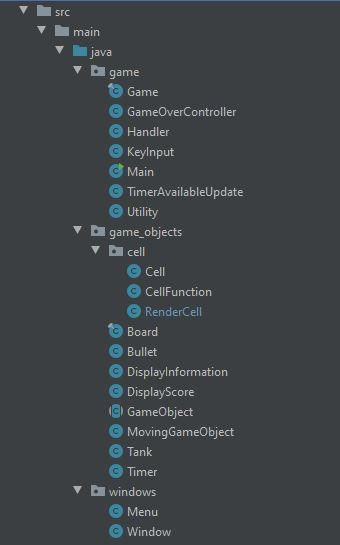
\includegraphics[width=7cm,center]{images/klasy_w_pakietach.JPG}
    \captionof{figure}{Zawartość trzech głównych pakietów}
\end{figure}

Pod-pakiet pakietu game\_objects o nazwie cell zawiera klasy zawierające funkcje potrzebne w Cell (pozwoliło to na zmniejszenie ilości linii kodu w tej klasie).

Dane są zapisane w folderze resources:
\begin{figure} [hbt!]
    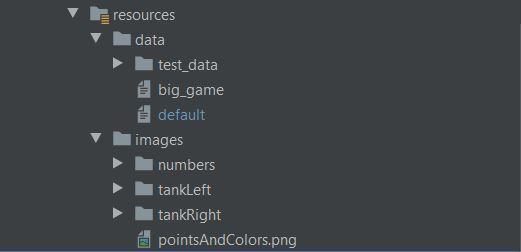
\includegraphics[width=7cm,center]{images/resources.JPG}
    \captionof{figure}{Zawartość folderu resources}
\end{figure}

\clearpage

\subsection{Diagram klas}
Uproszczony diagram klas, który zawiera same połączenia:
\begin{figure} [hbt!]
    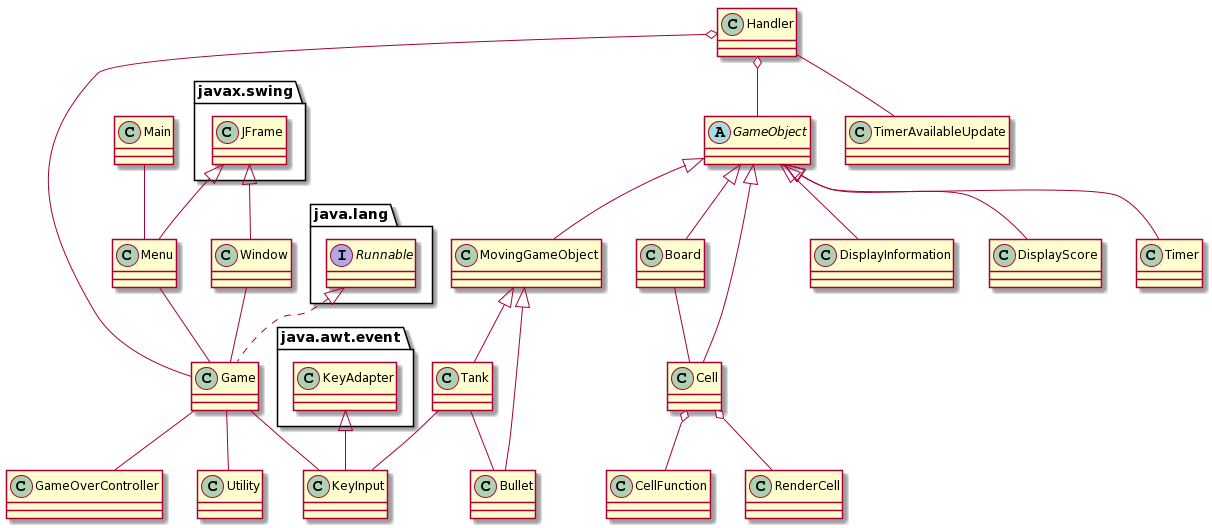
\includegraphics[width=20cm,center]{images/diagram_same_pol.png}
    \captionof{figure}{Diagram klas - połączenia}
\end{figure}

Zmienne statyczne w Game (np. P, H, ..., HEIGHT, WIDTH) są używane przez wiele klas: Utility, TimerAvailableUpdate, Cell, Board, Bullet, Tank, Timer.
Podobna sytuacja jest z Board.x, Board.y, Board.width. Istnieją także ciągi wywołań np. Main tworzy Menu, Menu tworzy Game. To wszystko tworzy dużą liczbę połączeń, dlatego zdecydowaliśmy się diagram uprościć.
\clearpage

\par Przedstawimy także jakie metody ma poszczególna klasa (uwzględniając atrybuty wykres robi się nieczytelny):

%\begin{figure} [hbt!]
    %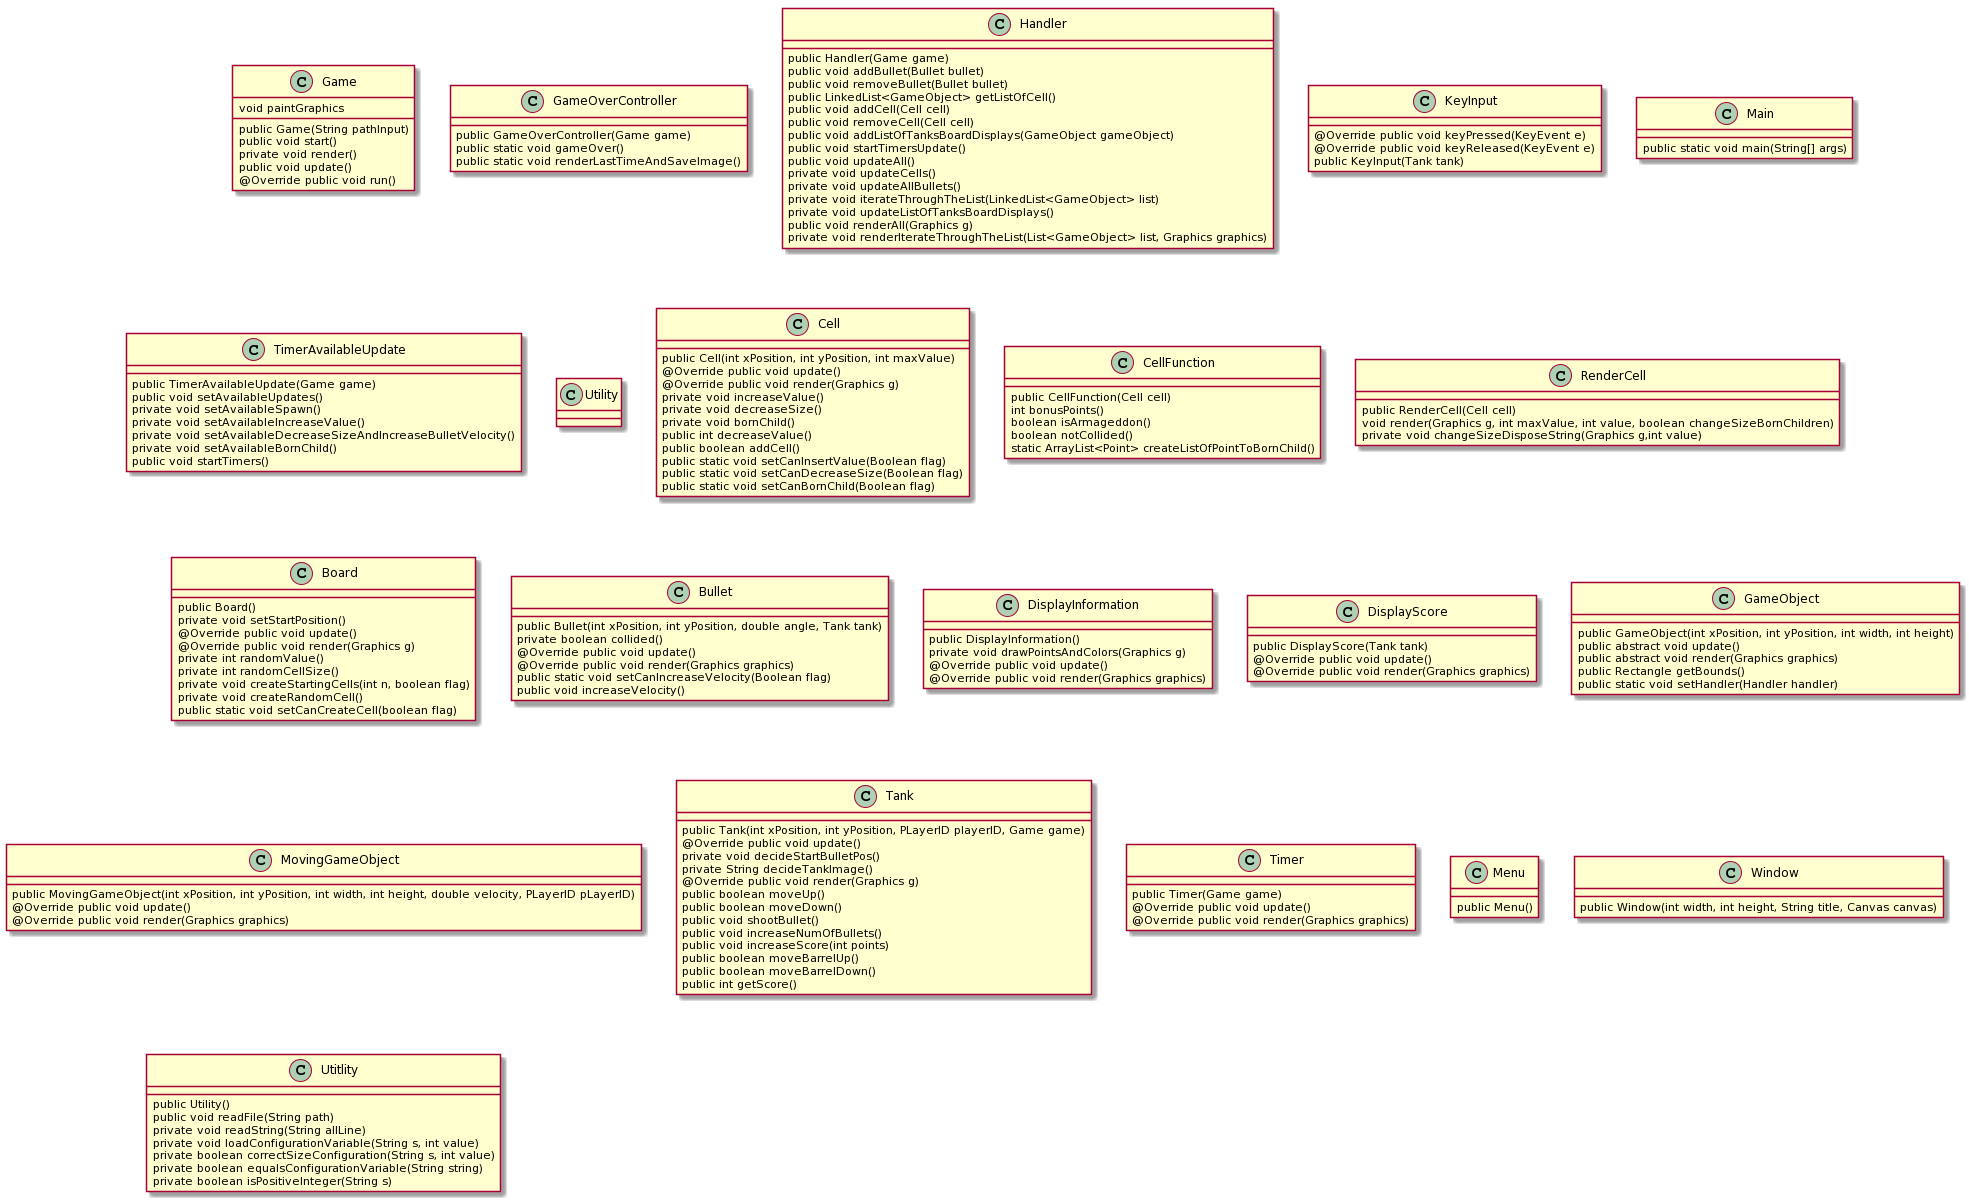
\includegraphics[width=20cm,center]{images/diagram_same_metody.png}
    %\captionof{figure}{Diagram klas - metody}
%\end{figure}

\begin{figure} [hbt!]
    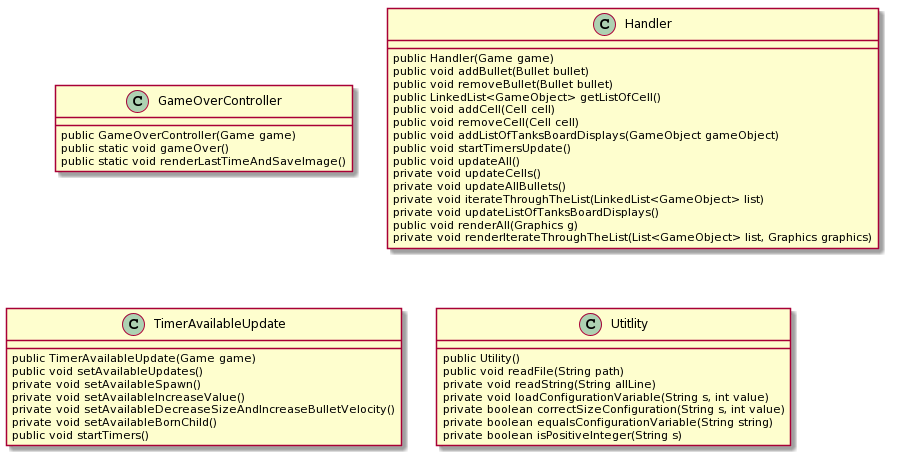
\includegraphics[width=15cm,center]{images/pakiet_game.png}
    \captionof{figure}{Diagram klas - pakiet game}
\end{figure}

\begin{figure} [hbt!]
    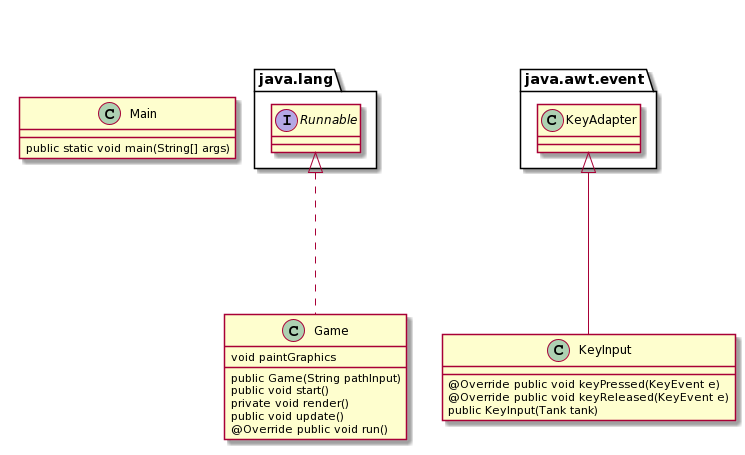
\includegraphics[width=13cm,center]{images/pakiet_game_cd.png}
    \captionof{figure}{Diagram klas - pakiet game}
\end{figure}

\begin{figure} [hbt!]
    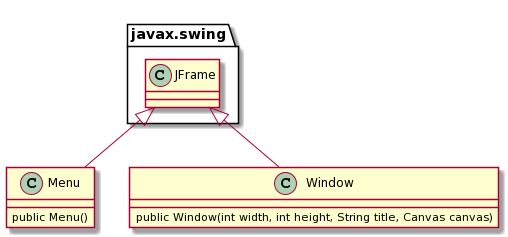
\includegraphics[width=12cm,center]{images/pakiet_window.png}
    \captionof{figure}{Diagram klas - pakiet window}
\end{figure}

\begin{figure} [hbt!]
    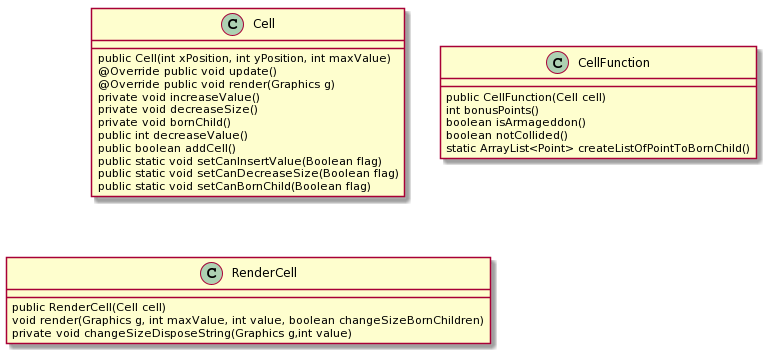
\includegraphics[width=15cm,center]{images/pakiet_cell.png}
    \captionof{figure}{Diagram klas - pakiet cell}
\end{figure}

\begin{figure} [hbt!]
    \includegraphics[width=13cm,center]{images/pozostałe_elelementy_game_object_1.png}
    \captionof{figure}{Diagram klas - pozostałe elementy game\_objects}
\end{figure}

\begin{figure} [hbt!]
    \includegraphics[width=13cm,center]{images/pozostałe_elelementy_game_object_2.png}
    \captionof{figure}{Diagram klas - pozostałe elementy game\_objects}
\end{figure}

\clearpage

\subsection{Użyte importy}
Korzystaliśmy głównie z bibliotek java.awt i javax.swing. Większość importów powtarza się w klasach, dlatego tutaj przedstawione są wszystkie różne importy.
\begin{itemize}
\item import java.awt.Canvas;
\item import java.awt.Color;
\item import java.awt.Graphics;
\item import java.awt.image.BufferStrategy;
\item import java.io.IOException;
\item import javax.imageio.ImageIO;
\item import javax.swing.JOptionPane;
\item import java.awt.image.BufferedImage;
\item import java.io.FileOutputStream;
\item import java.util.ArrayList;
\item import java.util.LinkedList;
\item import java.util.List;
\item import java.awt.event.KeyAdapter;
\item import java.awt.event.KeyEvent;
\item import java.io.BufferedReader;
\item import java.io.InputStreamReader;
\item import java.awt.Point;
\item import java.util.Collections;
\item import java.util.Random;
\item import java.awt.Font;
\item import java.awt.FontMetrics;
\item import java.awt.Rectangle;
\item import javax.swing.JButton;
\item import javax.swing.JFrame;
\item import javax.swing.JPanel;
\item import javax.swing.JTextField;
\item import java.awt.event.ActionEvent;
\item import java.awt.event.ActionListener;
\end{itemize}

Importy w klasie UtilityTest:
\begin{itemize}
    \item import org.assertj.core.api.Assertions;
    \item import org.junit.Before;
\item import org.junit.Test;
\end{itemize}

\subsection{Testy}
Utworzyliśmy jeden plik testowy UtilityTest (testujący klasę Utility).
Używamy w nim Assertions.assertThat (import org.assertj.core.api.Assertions).
Importujemy także:
\begin{itemize}
    \item org.junit.Before
    \item org.junit.Test
    \item org.junit.Assert.assertFalse
\end{itemize}

Dlatego w naszym pom.xml (Mavenowym) mamy:
\begin{minted} {xml}
    <dependencies>
        <dependency>
            <groupId>org.assertj</groupId>
            <artifactId>assertj-core</artifactId>
            <version>3.11.1</version>
            <scope>test</scope>
        </dependency>

        <dependency>
            <groupId>junit</groupId>
            <artifactId>junit</artifactId>
            <version>4.11</version>
            <scope>test</scope>
        </dependency>
    </dependencies>
\end{minted}

\clearpage

\subsection{Plik wejściowy}
Zawsze wczytujemy na początku plik wejściowy default:

\begin{figure} [hbt!]
    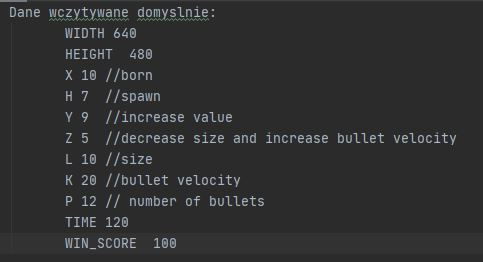
\includegraphics[width=12cm,center]{images/default.JPG}
    \captionof{figure}{Plik default}
\end{figure}

Następnie jeżeli użytkownik poda ścieżkę do innego pliku z parametrami gry, zostaną one zmienione. Przykładowo:

\begin{figure} [hbt!]
    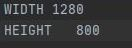
\includegraphics[width=5cm,center]{images/plik_przykladowy.JPG}
    \captionof{figure}{Plik big\_game}
\end{figure}

Rozwiązanie to nie zadowoli w pełni użytkownika, ponieważ musi on podać ścieżkę do istniejącego już pliku (który znajduje się folderze data).

Zmienne, które użytkownik może ustawić to:
WIDTH, HEIGHT, X, H, Y, Z, L, K, P, TIME, WIN\_SCORE. Ograniczamy WIDTH i HEIGHT do rozmiarów (kolejno): <480, 1440> oraz <360, 1080>.

\clearpage

\subsection{Plik wyjściowy}
Po zakończeniu gry poprzez koniec czasu lub wygraną gracza, gra zapisuje stan planszy w postaciu pliku PNG.
\begin{figure} [hbt!]
    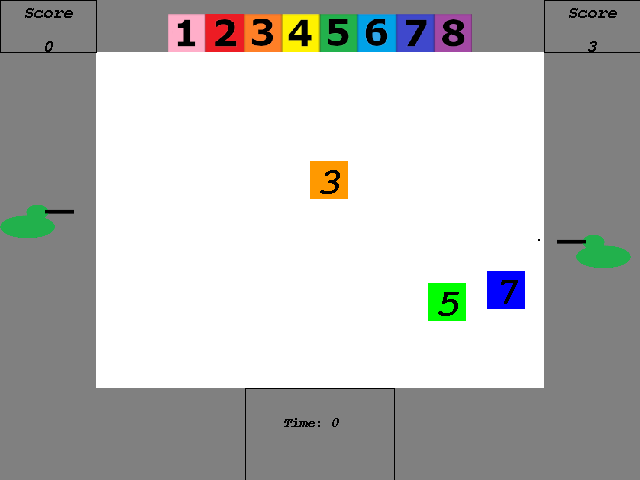
\includegraphics[width=15cm,center]{images/WindowsGameOverScreen.png}
    \captionof{figure}{Koniec gry przez upłynięcie czasu}
\end{figure}

Zapisuje się on w miejscu: Game\_of\_tanks \slash kod\slash GameOverScreen.png przez uruchomienie gry przez środowisko (Intellij'a ) lub w: Game\_of\_tanks \slash kod\slash target\slash GameOverScreen.png przez uruchomienie gry za pomocą jara.
\clearpage

\section{Podsumowanie współpracy} 

\subsection{Środowisko pracy}
Nie zmienialiśmy naszych środowisk pracy, pozostaliśmy przy IntelliJ IDEA 2020.1. Używaliśmy javy 14 w projekcie w Intellij'u i na naszych komputerach (np. przy java -jar przez terminal).

\par Pozostaliśmy przy pisaniu gry na dwóch różnych systemach operacyjnych: Ubuntu 19.10 i Windows 10. Powoduje to małe różnice w wyglądzie JFrame'a - aplikacji z grą.

\subsubsection{Różnice w grze}
\begin{figure} [hbt!]
    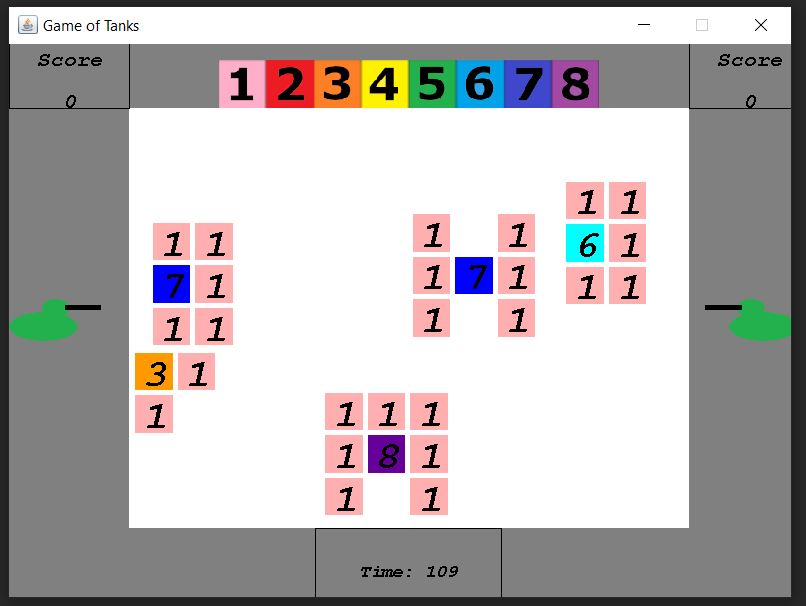
\includegraphics[width=15cm,center]{images/windowsApp.jpg}
    \captionof{figure}{Gra działająca na Windowsie}
\end{figure}

\clearpage

\begin{figure} [hbt!]
    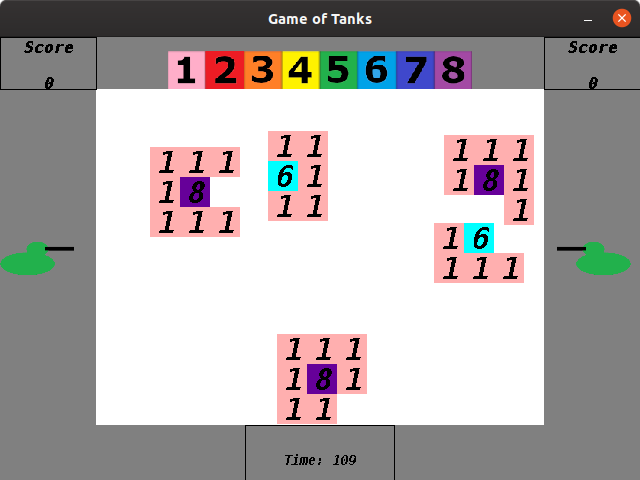
\includegraphics[width=15cm,center]{images/UbuntuApp.png}
    \captionof{figure}{Gra działająca na Ubuntu}
\end{figure}

%\clearpage
%\clearpage

\subsubsection{Praca z gitem}
Utworzyliśmy 9 gałęzi (nie licząc gałęzi 10., którą utworzymy aby wrzucić to sprawozdanie) o nazwach (jedna gałąź została nazwana przypadkowo po polsku zamiast po angielsku, nie udało nam się tego zmienić):
\begin{itemize}
    \item 1\_Specifications  
    \item 2\_runLoop  
    \item 3\_Change\_of\_Folder\_Structure
    \item 4\_creating\_Board  
    \item 5\_Adding\_Maven\_and\_Tests\_to\_Project  
    \item 6\_Tanks\_and\_bullets  
    \item 7\_Second\_Tank\_and\_Display  
    \item 8\_Utility\_and\_Menu  
    \item 9\_Jar\_and\_project\_structure 
\end{itemize}
Finalna wersja znajduje się na gałęzi master.

Jako, że robiliśmy dwa projekty na jednym repozytorium to pozostałe gałęzie oraz folder ,,PROJEKT GRA W ZYCIE'' odnosi się do pierwszego projektu (Gra w Życie w języku programowania C).

%\clearpage

\section{Uruchomienie programu}

\subsection{Menu}
Pierwsze co włącza się po uruchomieniu gry to Menu z trzema przyciskami:
\begin{figure} [hbt!]
    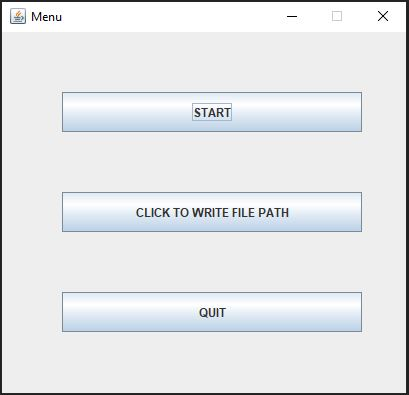
\includegraphics[width=8cm,center]{images/menu.JPG}
    \captionof{figure}{Menu}
\end{figure}

\begin{itemize}
    \item Przycisk ,,QUIT'' wychodzi z Menu (także z całej gry).
    \item Przycisk ,,START'' staruje grę.
    \item Po naciśnięciu przycisku ,,CLICK TO WRITE FILE PATH'' pojawia się pole, w którym możemy wpisać ścieżkę do pliku. Dodatkowo musi ona wyglądać tak: ,,/data/nazwa\_pliku'' (plik jest w folderze data).
    
    \clearpage
    
    \begin{figure} [hbt!]
    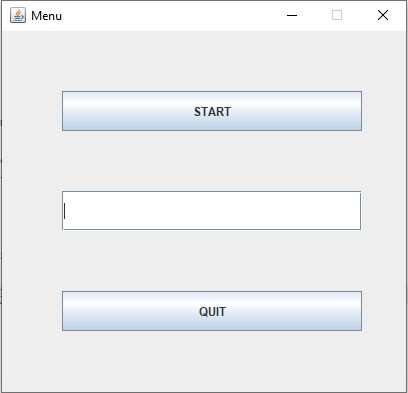
\includegraphics[width=8cm,center]{images/menu_path.JPG}
    \captionof{figure}{Przycisk CLICK TO WRITE FILE PATH}
    \end{figure}
    
    \begin{figure} [hbt!]
    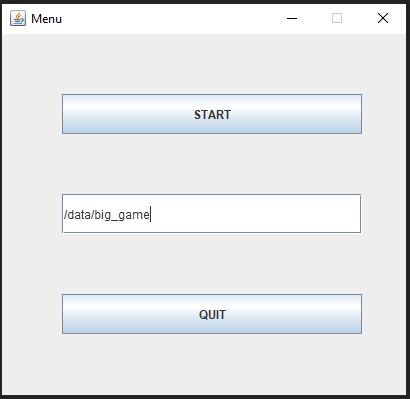
\includegraphics[width=8cm,center]{images/menu_path2.JPG}
    \captionof{figure}{Wpisanie ścieżki }
    \end{figure}
    
\end{itemize}

\subsection{Jak włączyć grę}
\begin{enumerate}
    \item Wpisanie ,,java -jar Game\_of\_tanks-1.0-SNAPSHOT-jar-with-dependencies.jar,, w konsoli (będąc w folderze target projektu).
    \item Kliknięcie 2 razy na plik jar.
\end{enumerate}

\subsection{Przedstawienie reakcji na błędy}
Jeżeli ścieżka do pliku będzie wskazywać na nieistniejący plik lub nie będzie poprzedzona ,,/data/'' to program uruchomi się z wartościami z pliku domyślnego.\\
Aplikacja najpierw wczytuje dane domyślne dane (/data/default). Jeśli w pliku wejściowym poprawnie będzie podana dana konfiguracja (np. P 20) to ją nadpisuje. Inne połączenia/znaki niż nazwy zmiennych z liczbami ignoruje.

\subsection{Sytuacje wyjątkowe}
Błędy, na które nie mamy wpływu to:
\begin{itemize}
    \item Jeżeli program nie wczyta pliku konfiguracyjnego domyślnego (default) to na konsoli wypisze się błąd i należy uruchomić ponownie program (jedynie przez uruchomienie za pomocą Intellij'a - niestety ten błąd będzie niezauważony podczas włączenia gry przez jara).
    \item Jeśli nie pojawi się czołg lub obraz z punktacją to na konsoli wypisze się błąd, ale będzie można kontynuować grę (bez wyświetlanego czołgu - pozycja pocisków czy zdobywanie punktów nadal działa).
\end{itemize}
\par Dodatkowo przy dużej ilości komórek na planszy gra może się zacinać.

\section{Wnioski po wykonaniu projektu}
Projekt udało się wykonać mimo braku doświadczenia w Javie (zdobywaliśmy go w trakcie trwania projektu). \\
Do poprawy jest wczytywanie pliku konfiguracyjnego (aby użytkownik mógł wprowadzić plik ze swojego komputera - taki który nie jest załadowany do jara) oraz napisanie więcej testów jednostkowych. \\
Lepiej by było zacząć projekt od razu z Mavenem oraz lepszym rozwiązaniem graficznym byłby javaFx, z którym też byśmy zaczęli projekt (nowy projekt w Intellij'u za pomocą Mavena i JavyFx).

\subsection{Wnioski z Proof of Concept}
Wszystkie zadania wyznaczone w sprincie trwającym do Proof of Concept udało nam się zrealizować oprócz pliku jara, który wykonaliśmy w następnym sprincie. Także zadania z drugiego sprintu udało nam się wszystkie zrealizować.

\subsection{Co można by usprawnić w działaniu programu} 
\begin{itemize}
    \item Pracować z javaFx.
    \item Użyć Timerów i TimerTasków zamiast implements Runnable (brak funkcji run i w niej pętli while).
    \item Renderować tylko konkretne komponenty zamiast całej planszy od nowa.
\end{itemize}

\subsection{Organizacja w zespole}
Przynajmniej raz w tygodniu rozmawialiśmy na temat projektu (przez platformę Teams) i ustalaliśmy zadania na kolejny tydzień, do których sami się do nich zgłaszaliśmy. Obydwoje nie ma mamy zastrzeżeń do współpracy.

\section{Źródła}
\begin{itemize}
    \item Diagramy klas: \\
    https://www.p-programowanie.pl/uml/diagramy-klas-uml/ \\
    http://zasoby.open.agh.edu.pl/~09sbfraczek/diagram-klas\%2C1\%2C11.html
    
    \item Diagram klas wykonany za pomocą https://plantuml.com/class-diagram
    
    \item Opis teoretyczny został przedstawiony przez dr. Pawła Zawadzkiego
    
    \item Ten dokument został utworzony w LaTeX'ie za pomocą strony https://www.overleaf.com
    
    \item  Jest to trzeci z kolei i ostatni dokument dotyczący projektu ,,Game\_of\_tanks''
    
    \item Początkowa inspiracja: \\
        https://marcusman.com/ oraz 
        ,,Java Programming: Let’s Build a Game by RealTutsGML''
\end{itemize}

\end{document}